\documentclass{article}
\usepackage{mathmag}

\usepackage{amsmath,amsthm}
\usepackage{graphicx}
\usepackage{hyperref}
\usepackage{url}
\usepackage{amsfonts}

\usepackage{multicol}


% NOTE mathmag.sty calls the text fonts. For this template we are using times.sty
% from the standard LaTeX distribution.

%% IF YOU HAVE FONTS INSTALLED you can use these math fonts to more
%% closely approximate the final product.
%\usepackage{mtpro2}
%\usepackage{mathtime}

\theoremstyle{theorem}
\newtheorem{theorem}{Theorem}

\theoremstyle{definition}
\newtheorem*{definition}{Definition}
\newtheorem*{remark}{Remark}

\allowdisplaybreaks

\makeatletter
\@addtoreset{footnote}{page}
\makeatother

%%%%%%%%%%%%%%%%%%%%%%%%%%%%%%%%%%%%%%%%%%%%%%%%%%
\begin{document}

\title{Segregation Surfaces}

\author{Author Name\\               %%%% Leave ALL of these as is in your initial submission
\scriptsize affiliation line 1\\    %%%% to allow for double blind reviewing.
affiliation line 2\\                %%%% They should be filled in when you are submitting
email address}                      %%%% your final manuscript.

\maketitle

\noindent Over the past half century, social scientists have devised a clever assortment of tools to measure the nature and extent of segregation. \cite{harrisjohnson18} Usually, a segregation measurement takes the form of a number, or \textit{index}, which quantifies the isolation and clustering of groups defined by race, income, education, or other factors. Numerical indices are handy because they can give us ways to track changes in a neighborhood over time, and they allow for comparisons among different regions.

However, numerical summary statistics alone are limited when it comes to finding geometric patterns of segregation in two-dimensional data. In this note, we use some familiar ideas from third-semester calculus to extend the machinery behind some commonly-used segregation indexes. We will see how segregation patterns can be represented by a surface, and how the geometric properties of these surfaces reveal ways that our cities and towns are divided.

\section{Numerical measures of segregation.}

In order to define a segregation measure, we assume that we have data describing the population within a particular geographic region, including the locations of where people live. For simplicity, we will regard the population as being split into two sets $A$ and $B$, where $B$ is the complement of $A$ (e.g., white/nonwhite, above/below median income). Most of the measures we consider below can be extended to more than two groups.

One of the earliest measures of segregation to become widely adopted is the \textit{index of dissimilarity} of Duncan and Duncan. \cite{duncan55} The definition of this index requires a partition of region in question into $k$ subsets; typically, this partition is defined by census tracts or block groups. For each subset of this partition, let $a_i$ be the population of group $A$ residing the the subset, and let $b_i$ be the population of group $B$, where $1 \leq i \leq k$. Denote the total populations of groups $A$ and $B$ by $N_A$ and $N_B$, respectively. The index of dissimilarity $D$ is then given by summing the absolute differences of the proportions of each group living in each subset.

\begin{equation}
  D = \frac{1}{2} \sum_i \left\lvert \frac{a_i}{N_A} - \frac{b_i}{N_B} \right\rvert
\end{equation}

If our two groups were evenly distributed, we would expect to see similar proportions of each in every subset, resulting in a value of $D$ near zero. On the other hand, if our region were completely segregated, each subset would contain zero of one group, so the above summation would simply tally up the proportions of each, resulting in $D = 1$.

The index of dissimilarity has two glaring weaknesses. First, it is highly sensitive to how the subsets are defined. A different allocation of census tracts could result in a different value of $D$. Second, it suffers from the so-called ``checkerboard problem.''~\cite{morrill91} To illustrate this second issue, consider the three different segregation patterns in Figure~\ref{fig:checkerboard}. Suppose that $N_A = N_B$ and that each of the 32 rectangular subsets contains the same number of residents. For a fixed proportion $p$, suppose that $p$ of each shaded subset is from group $A$ and $1-p$ is from group $B$, while $p$ of each non-shaded region is from group $B$ and $1-p$ from group $A$. It is easy to check that $D = \lvert 2p-1 \rvert$ in all three cases, even though the first pattern seems objectively more segregated than the third.

\begin{figure}\centering
  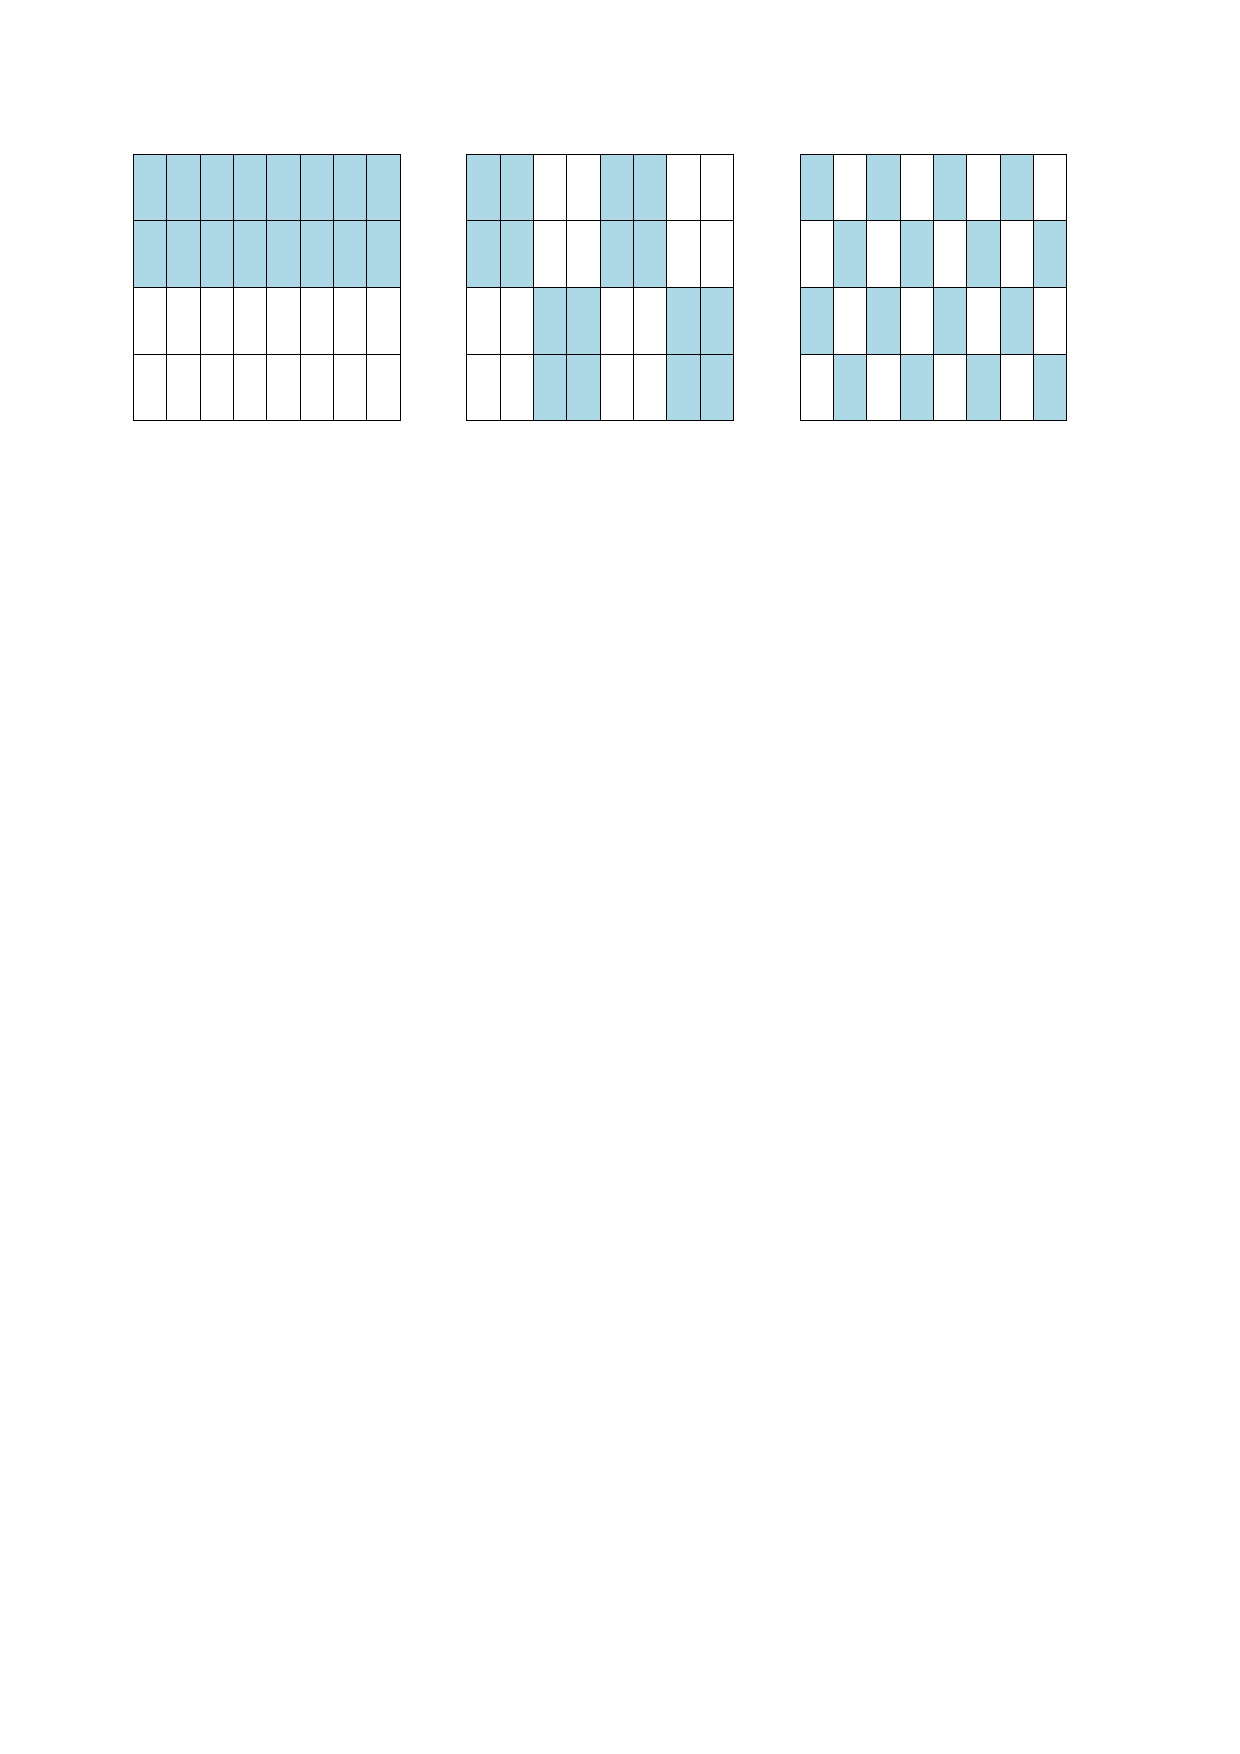
\includegraphics[width=4in]{checkerboard.pdf}
  \caption{Three different segregation patterns with the same index of dissimilarity.}
  \label{fig:checkerboard}
\end{figure}

To address these two weaknesses, O'Sullivan and Wong \cite{osullivanwong07} propose a generalization of $D$ using surfaces. Let $a(x,y)$ and $b(x,y)$ be two-dimensional probability density functions describing the distribution of groups $A$ and $B$, respectively, in our region~$R$. The segregation index $S$ is then defined as
\begin{equation}\label{eqn:S1}
  S = 1 - \frac{V_\cap}{V_\cup},
\end{equation}
where $V_\cap$ and $V_\cup$ are the volumes of the intersection and union of the solid regions above the $xy$-plane and below the surfaces $z = a(x,y)$ and $z=b(x,y)$. In other words, these volumes are given by
\begin{equation}\label{eqn:S2}
  V_\cap = \iint_R \min(a, b) \, dA \quad \text{ and } \quad V_\cup = \iint_R \max(a,b) \, dA.
\end{equation}

If groups $A$ and $B$ are identically distributed, then $V_\cap$ will equal $V_\cup$, resulting in $S = 0$. However, more segregation will tend to reduce the volume $V_\cap$ under both surfaces relative to the total volume $V_\cup$, yielding values of $S$ closer to~1.

For example, consider the segregation patterns in Figure~\ref{fig:checkerboard}, letting the region $R$ be the square $[0,1] \times [0,1]$, and suppose that $0.5 < p \leq 1$. Suppose that $a(x,y)$ is a piecewise constant density function, taking the value $2p$ in the shaded regions and $2(1-p)$ in the non-shaded regions. (The top row of graphs in Figure~\ref{fig:kdeexamples} shows the density functions $a(x,y)$ corresponding to the three segregation patterns.) Similarly, let $b(x,y)$ take the value $2(1-p)$ in the shaded regions and $2p$ in the non-shaded regions. Using Equations~\ref{eqn:S1} and~\ref{eqn:S2}, we obtain $V_\cap = 2(1-p)$ and $V_\cup = 2p$, giving $S = (2p-1)/p$ for all three patterns. So it appears that this measurement also has the checkerboard problem.

However, it is somewhat unreasonable to assume that the true density functions that describe our population would be piecewise constant. Instead, O'Sullivan and Wong approximate $a$ and $b$ by smooth surfaces $\hat{a}$ and $\hat{b}$ using \textit{kernel density estimation}. A kernel density estimate is a smooth function that approximates a probability density based on a set of data points. \cite{wandjones11} In our case, this estimate is a weighted sum of 32 bivariate normal distributions, each centered on one of 32 rectangles that make up our region. There are lots of different ways to construct kernel density estimates; see \cite{wandjones11} and \cite{dengwickham11} for details.

Figure~\ref{fig:kdeexamples} shows the graphs of density functions for the three patterns in Figure~\ref{fig:checkerboard}, using $p = 0.8$. The top row shows the corresponding three piecewise-constant density functions $a$, while the bottom row shows the smoothed versions $\hat{a}$. (The functions $b$ and $\hat{b}$ are similar.) The smoothing has the effect of eliminating the checkerboard problem. While Equations~\ref{eqn:S1} and~\ref{eqn:S2} yield $S = 0.75$ using all three piecewise-constant versions of $a$ and~$b$, their smooth counterparts $\hat{a}$ and $\hat{b}$ give $S$-values of 0.68, 0.37, and 0.05, respectively.
% these numbers are generated in checkersurf.Rmd
It is important to note that these results are not uniquely determined. The surfaces, and the values of $S$ they produce, depend on the choice of kernel estimator and on adjustable smoothing parameters. More on this later.

\begin{figure}
  \includegraphics{checkersurf.pdf} % generated by checkersurf.Rmd
  \caption{The top row shows the three piecewise constant density functions corresponding to the patterns in Figure~\ref{fig:checkerboard}. The bottom row shows smoothed versions obtained using kernel density estimation.}
  \label{fig:kdeexamples}
\end{figure}

There are lots of other measures of segregation. Good summaries of the literature include \cite{reardonosullivan04}, \cite{harrisjohnson18}, and \cite{yao18}. All of these measures summarize the segregation patterns in a given region by a number---usually an index between zero and one. In the next section, we will consider how to go beyond these numerical summaries and create visualizations of segregation patterns using the geometric properties of the surfaces that define some of the commonly-used segregation indexes.

\section{Drawing segregation boundaries.}

\begin{figure}\centering
  \includegraphics{baltimoreqp.pdf}
  \caption{Choropleth map of Baltimore, Maryland, with superimposed contours. Census block groups are shaded according to the proportion of white residents. The contour lines show levels of the estimated conditional probability $\hat{f}(x,y)$ that a resident is white, given that the resident lives at point $(x,y)$.}
  \label{fig:choropleth}
\end{figure}

Given geographic data on where the members of two groups $A$ and $B$ live, is it possible to discern boundaries between neighborhoods where the residents are mostly from group $A$ and neighborhoods where the majority are from group $B$? In terms of probability, we would like to determine the set of points $(x,y)$ where, if you were to encounter a resident, the probability that the resident is from group $A$ is 0.5. In other words, we need to calculate a conditional probability.

As above, let $a(x,y)$ and $b(x,y)$ be the probability density functions that describe the distribution of groups $A$ and $B$ in our region. In addition, let $u(x,y)$ be the probability density function that describes the distribution of the entire population $U$, the disjoint union of $A$ and $B$. Using Bayes' Theorem, the conditional probability $f(x,y)$ that a resident belongs to group $A$, given that the resident lives at point $(x,y)$, is given by
\begin{equation}\label{eqn:f}
  f(x,y) = \frac{\lvert A\rvert\cdot a(x,y)}{\lvert U\rvert \cdot u(x,y)}\text{.}
\end{equation}
The 50\% contour of $f(x,y)$ will then be the border between a majority $A$-neighborhood and a majority $B$-neighborhood.\footnote{A function similar to $f$ appears in \cite{reardonosullivan04}, though it is motivated and defined differently, and allows for a distinction between geometric proximity and sociological proximity. Their function $\tilde{\pi}_{pm}$ represents ``the population composition that a person living at point $p$ would experience in his or her local environment.''}

In practice, the functions $a$, $b$, and $u$ can be estimated from data using kernel density estimation. Suppose that we have population counts for the $n$ subsets in a partition of our region (e.g., census block groups). Let $(x_i, y_i)$ be the centroids of each of these subsets, and assign weights $w_i$ to each subset based on the population counts, such that $\sum w_i = n$. We then can estimate $u$ as
$$
\hat{u}(x,y) = \frac{1}{n} \sum_{i=1}^n w_i K\left(\frac{x-x_i}{h_x}, \frac{y-y_i}{h_y} \right)\text{,}
$$
where $K(x,y)$ is a bivariate normal kernel function, and $h_x, h_y$ are smoothing parameters, or \textit{bandwidths}. Estimates $\hat{a}$ and $\hat{b}$ for $a$ and $b$ are defined similarly, and then Equation~\ref{eqn:f} gives an estimate $\hat{f}$.

Figure~\ref{fig:choropleth} illustrates the result of this construction using census block group-level data on the proportion of white residents in Baltimore, Maryland. Each census block is shaded according to the proportion of white residents, forming a \textit{choropleth} map. The contour lines show levels of $\hat{f}(x,y)$, which estimates the probability that a resident is white, given that the resident lives at point $(x,y)$. Since this probability is constant along these contours, we expect each curve to pass through regions with similar shading.

The choice of smoothing parameters $h_x, h_y$ greatly affects the geometry of the surface $z = \hat{f}(x,y)$ and its contours. Small values produce very bumpy surfaces that closely fit the data points, while large values give smooth surfaces that loosely approximate the data points. Figure~\ref{fig:overunderfit} shows the 50\% contours of $\hat{f}$ for three different choices of smoothing parameters, using the same data as in Figure~\ref{fig:choropleth}, but with each shaded region replaced by its centroid. The plot on the left appears to be \textit{undersmoothed}, because the very wiggly contours give neighborhood boundaries that are overly sensitive to particular data points. On the other hand, the plot on the right is \textit{oversmoothed}, because the contours fail to capture the granularity in the data.

\begin{figure}
  \includegraphics{overunderfit.pdf}
  \caption{Fifty-percent contours of $\hat{f}$ for three choices of smoothing parameters. The left plot shows undersmoothing, while the right plot shows oversmoothing.}
  \label{fig:overunderfit}
\end{figure}

\section{The segregation gradient.}

In addition to locating segregation boundaries, the surface $z = \hat{f}(x,y)$ can identify the rate at which population proportions change with respect to distance. In particular, the \textit{segregation gradient} $\nabla \hat{f}(x,y)$ gives the magnitude and direction of this change.

Plotting segregation gradients on a map of a region can highlight geographic features that affect how segregated neighborhoods form. For example, Figure~\ref{fig:chicagowest} shows racial segregation patterns in the near-west suburbs of Chicago, where $A$ is the set of white residents, and $B$ is the set of nonwhite residents, according to data from the 2017 American Community Survey (ACS). Areas with large segregation gradients correspond to neighborhoods where the racial composition changes markedly over a short distance. For example, the vertical green strip about a third of the way from the left is a forest preserve. The eastward pointing segregation gradients suggest that the neighborhoods to the east of this forest are predominately white, in contrast to some of the neighborhoods to the west.

\begin{figure}
  \includegraphics{chicagowest.pdf}
  \caption{White/non-white segregation gradients in the near-west suburbs of Chicago. The arrows indicate the directions in which the proportion of white residents increases. The longer the arrow, the more sudden the change.}
  \label{fig:chicagowest}
\end{figure}

The magnitude of the segregation gradient can quantify the severity of segregation in a given location. In particular, along the 50\% contours that divide majority $A$ neighborhoods from majority $B$ neighborhoods, the segregation gradient indicates how fast these neighborhoods change from $A$ to $B$. For example, Figure~\ref{fig:sanfran1317} shows two maps of income segregation in San Francisco, CA, using ACS data from 2013 and 2017. In these data sets, group $A$ consists of residents whose income is above the county median, while group $B$ contains residents with below-median income. The thickness of the 50\% contour lines corresponds to the magnitude of the segregation gradient. Thin contour lines indicate a gradual change in the income of the residents, while thick contour lines indicate stark divisions. In both maps, the thickest contour is in the southeast corner, separating the India Basin neighborhood from the more popular Central Waterfront neighborhood to the north.

Figure~\ref{fig:sanfran1317} also shows how income segregation has changed in San Francisco from 2013 to 2017. In the 2013 plot on the left, the small closed curves enclose lower-income (group $B$) neighborhoods. In the 2017 data, these areas of below-median income have vanished, and the large region in the middle populated by higher-income residents has expanded. These trends in the data are consistent with anecdotal observations of gentrification in San Francisco. \cite{pogash15}

\section{Measuring segregation with gradients.}

In relatively integrated regions, we would expect the magnitude of the segregation gradient to be small, on average, along the 50\% contours. In regions where groups $A$ and $B$ tend to cluster together (such as in Figure~\ref{fig:chicagowest}), the magnitude $\lVert \nabla \hat{f} \rVert$ will exhibit more variability. So we can define a new segregation index $G_C$ by averaging the value of  $\lVert \nabla \hat{f} \rVert$ along the 50\% contour $C$ of a region. Since segregation indexes are traditionally numbers between zero and one, we use the arctangent function to convert this average from a slope to an angle.
\begin{equation}\label{eqn:gc}
   G_C = \frac{2}{\pi} \arctan \left(\frac{1}{\mathrm{length}(C)} \int_C \lVert \nabla \hat{f} \rVert \, ds \right)
\end{equation}
Applying this formula to the three segregation patterns in Figure~\ref{fig:checkerboard}, we obtain the values $G_C=0.79$, $G_C=0.65$, and $G_C=0.13$, respectively.
% these values are computed in checkersurf.Rmd

\begin{figure}
  \includegraphics{sanfran1317.pdf} % generated in gradientplots1317.Rmdneighborhoods
  \caption{Gentrification in San Francisco. Income segregation patterns have changed from 2013 (left) to 2017 (right). The contours enclose neighborhoods whose residents tend to have incomes below the county median. Some of these neighborhoods have been shrinking. Thicker contours represent starker divisions.}
  \label{fig:sanfran1317}
\end{figure}

Of course, Equation~\ref{eqn:gc} only makes sense if our function $\hat{f}$ takes the value 0.5 somewhere in its domain. For example, in Figure~\ref{fig:sanfran1317}, we ensure that this will happen by taking groups $A$ and $B$ to be the same size. In a region with where, say, group $A$ is much larger than group $B$, and the members of group $B$ are fairly well dispersed, there may fail to be any points on the 50\% contour $C$. In this situation, $G_C$ would be undefined. When applying Equation~\ref{eqn:gc} to data, the lack of a contour $C$ is usually an indication that there is not much diversity in terms of the groups $A$ and $B$.

The problem of a nonexistent 50\% contour can be avoided by averaging the magnitude of the gradient across the entire region, without regard to neighborhood boundaries. Doing so gives us $G_R$, a second measure of segregation.
\begin{equation}\label{eqn:GR}
   G_R = \frac{2}{\pi} \arctan \left(\frac{1}{\mathrm{area}(R)} \iint_R \lVert \nabla \hat{f} \rVert \, dA \right)
\end{equation}
When applied to the patterns in Figure~\ref{fig:checkerboard}, Equation~\ref{eqn:GR} yields $G_R = 0.26$, $G_R = 0.56$, and $G_R = 0.16$, respectively. In this case, the first segregation pattern gives us a lower value of $G_R$ because the gradient is close to zero in the large homogeneous areas. On these artificial examples, it appears that $G_R$ underestimates segregation in highly-divided regions with relatively few clusters of each group.

How do $G_C$ and $G_R$ compare when applied to real data? On a sample of 74 large, racially diverse counties in the United States, $G_C$ and $G_R$ show a fairly strong correlation ($r \approx 0.8$), when computed using 2017 ACS data on race (white/nonwhite). A scatterplot of these 74 observations appears in Figure~\ref{fig:gcgrcor}. Regions with large values of both $G_C$ and $G_R$ tend to be large, established urban centers, while smaller values generally correspond to areas having a more suburban character. The unusual observations in this scatterplot illustrate the difference between $G_C$ and $G_R$. For example, Denver, Colorado has several small nonwhite clusters of population, but lacks large areas with starkly-defined borders. As a result, Denver has a fairly typical value of $G_R$, but a low $G_C$ value. On the other side of the trend line, Riverside, California has one or two nonwhite clusters among a large swath of majority white neighborhoods, resembling a version of the first pattern in Figure~\ref{fig:checkerboard}, where $G_R$ seems to underestimate the amount of segregation.

\begin{figure}
  \includegraphics{gcgrcor.pdf}
  \caption{A scatterplot showing the correlation between $G_C$ and $G_R$, when computed on 74 large, diverse US counties.}
  \label{fig:gcgrcor}
\end{figure}

Caution should be always be exercised when trying to quantify segregation, as there are many different types of patterns of division. Massey and Denton \cite{masseydenton88}  propose five ``dimensions'' of segregation: evenness, exposure, clustering, centralization, and concentration. Discussion and revisions of this framework can be found in \cite{johnston07} and \cite{brownchung06}. From another perspective, Reardon and O'Sullivan \cite{reardonosullivan04} argue in favor of two orthogonal continua, clustering--evenness and isolation--exposure. A notable lack of consensus still persists in the social science literature, and the multifaceted nature of the phenomenon has motivated a bewildering variety of measurements for it. \cite{harrisjohnson18}

We can test some of these measurements on our sample of 74 counties. Table~\ref{tab:indexcor} shows the pairwise correlations of the gradient measures $G_C$ and $G_R$, along with five other indexes: O'Sullivan and Wong's $S$ of Equation~\ref{eqn:S1}, the spatial dissimilarity index $\tilde{D}$, the spatial information theory index $\tilde{H}$, and the exposure/isolation index $\tilde{P}^*$, and the Geary ratio $C$. Three of these, $\tilde{D}$, $\tilde{H}$, $\tilde{P}^*$, are defined in \cite{reardonosullivan04} and implemented in \cite{hong14}. Geary's $C$ measures \textit{spatial autocorrelation} \cite{clifford81}, and is implemented in \cite{bivand19}. Since small values of $C$ indicate that neighboring block groups tend to be similar, $C$ is negatively correlated with the smooth dissimilarity index $S$, as well as to other measures of segregation.

\begin{table}[bh]
\centering
\begin{tabular}{l|rrrrrrr} % Computed in countyWhiteSeg.R
   & $G_C$ & $G_R$ & $S$ & $\tilde{D}$ &  $\tilde{H}$ & $\tilde{P}^*$ & $C$ \\
  \hline
  $G_C$ & 1.0 & 0.8 & 0.6 & 0.0 & 0.1 & 0.2 & -0.7 \\
  $G_R$ &  & 1.0 & 0.5 & -0.1 & 0.3 & 0.4 & -0.6 \\
  $S$ &  &  & 1.0 & 0.6 & 0.0 & 0.2 & -0.9 \\
  $\tilde{D}$ &  &  &  & 1.0 & 0.1 & -0.1 & -0.5 \\
  $\tilde{H}$ &  &  &  &  & 1.0 & 0.5 & -0.1\\
  $\tilde{P}^*$ &  &  &  &  &  & 1.0 & -0.2  \\
\end{tabular}
\caption{Correlation matrix for several different segregation measures, when computed on a sample of 74 large US counties.}
\label{tab:indexcor}
\end{table}


\section{Resources and questions for future investigation.}

All of the figures and calculations given in this note can be reproduced using the data and R code in the GitHub repository at
%\href{https://github.com/djhunter/segregation}{\url{https://github.com/djhunter/segregation}}.
\url{url.redacted.pending.review}. An enormous trove of ACS census data is readily available online \cite{acs19}, and convenient interfaces such as \cite{walker19} allow for its integration with geographic data.

Because of its interdisciplinary nature, the study of segregation naturally lends itself to student projects. Ideas for future undergraduate research problems include the following.

\begin{itemize}
  \item All of the examples considered above considered two groups, $A$ and $B$. Invent a way of visualizing segregation patterns involving more than two groups. How could you extend the definitions of $G_C$ and $G_R$ to this case?
  \item When studying population dynamics, we generally regard data as two-dimensional. However, our definition of $\hat{f}$ could easily be modified for domains that are subsets of $\mathbb{R}$ or $\mathbb{R}^3$.  Can you think of an application of segregation gradients using one- or three-dimensional data?
  \item In baseball, when the batter does not swing at a pitch, the home plate umpire decides whether the pitch is a ball or a strike. Ideally, umpires should call these pitches consistently. A consistent arrangement of called balls and strikes should look like a highly-segregated city, with a well-defined border between strikes (group $A$) and balls (group $B$). Can segregation indexes be used to assess umpire performance? Compare these measurements with those given in \cite{hunter18}.
  \item When computing $G_C$ and $G_R$, our function $\hat{f}$ was estimated from data. Compute these indexes for families of surfaces $z = f(x,y)$ for which you have analytic formulas. Are $G_C$ and $G_R$ related to other quantifiable properties of these surfaces (e.g., total curvature)?
  \item Ultrasound images consist of two-dimensional plots of the locations of reflected sound pulses, along with their intensities. Can the methods above for finding borders between neighborhoods be used to discern outlines of objects in these images, and quantify their sharpness? Investigate using raw data.
  \item Huff \cite{huff63} uses equiprobability contours of a certain surface to estimate the likelihood that residents from location $(x,y)$ will patronize a business at a given location. Given data on where clients of a given business reside, can we apply Bayes' Theorem (as in the construction of $\hat{f}(x,y)$) to obtain a similar estimating surface? Compare this approach to Huff's model.
\end{itemize}

\begin{thebibliography}{3}

\bibitem{bivand19} Bivand, R. (2019) spdep: Spatial Dependence: Weighting Schemes, Statistics. R package version 1.1-3. \href{https://cran.r-project.org/web/packages/spdep}{\url{https://cran.r-project.org/web/packages/spdep/}}

\bibitem{brownchung06}
Brown, L. A., Chung, S.-Y. (2006) Spatial segregation, segregation indices and the geographical perspective. \textit{Population, Space and Place.} 12(2): 125--143. doi:\href{https://doi.org/10.1002/psp.403}{10.1002/psp.403}

\bibitem{clifford81}
Cliff, A. D., Ord, J. K. (1982). \textit{Spatial processes: models and applications}, London: Pion.

\bibitem{dengwickham11} Deng, H., Wickham, H. (2011) Density Estimation in R. \href{https://vita.had.co.nz/papers/density-estimation.pdf}{\url{https://vita.had.co.nz/papers/density-estimation.pdf}}

\bibitem{duncan55} Duncan, D., Duncan, B. (1955) A Methodological Analysis of Segregation Indexes. \textit{American Sociological Review.} 20(2): 210--217. doi:\href{http://dx.doi.org/10.2307/2088328}{10.2307/2088328}

\bibitem{harrisjohnson18}
Harris, R., Johnson, R. (2018). Measuring and modelling segregation---New concepts, new methods and new data. \textit{Environment and Planning B: Urban Analytics and City Science.} 45(6): 999--1002. doi:\href{http://dx.doi.org/10.1177/2399808318808889}{10.1177/2399808318808889}

\bibitem{hong14} Hong, S., O'Sullivan, D., Sadahiro, Y. (2014). Implementing Spatial Segregation Measures in R. \textit{PLoS ONE}, 9(11): e113767. doi: \href{http://dx.doi.org/10.1371/journal.pone.0113767}{10.1371/journal.pone.0113767}

\bibitem{huff63} Huff, D. L. (1963). A Probabilistic Analysis of Shopping Center Trade Areas. \textit{Land Economics.} 39(1): 81--90. doi:\href{https://doi.org/10.2307/3144521}{10.2307/3144521}

\bibitem{hunter18} Hunter, D. (2018). New metrics for evaluating home plate umpire consistency and accuracy. \textit{Journal of Quantitative Analysis in Sports.} 14(4): 159--172. doi:\href{http://dx.doi.org/10.1515/jqas-2018-0061}{10.1515/jqas-2018-0061}

\bibitem{johnston07}
Johnston, R., Poulsen, M., Forrest, J. (2007). Ethnic and Racial Segregation in U.S. Metropolitan Areas, 1980--2000. \textit{Urban Affairs Review.} 42(4): 479--504. doi:\href{https://doi.org/10.1177/1078087406292701}{10.1177/1078087406292701}

\bibitem{masseydenton88} Massey, D., Denton, N. (1988). The Dimensions of Residential Segregation. \textit{Social Forces.} 67(2): 281--315. doi:\href{http://dx.doi.org/10.1093/sf/67.2.281}{10.1093/sf/67.2.281}

\bibitem{morrill91} Morrill, R. (1991) On the Measure of Geographic Segregation. \textit{Geography Research Forum.} 11: 25--36.

\bibitem{osullivanwong07} O'Sullivan, D., Wong, D. (2007). A Surface-Based Approach to Measuring Spatial Segregation. \textit{Geographical Analysis}, 39(2): 14--168. doi:\href{http://dx.doi.org/10.1111/j.1538-4632.2007.00699.x}{10.1111/j.1538-4632.2007.00699.x}

\bibitem{pogash15}
Pogash, C. (2015). Gentrification Spreads an Upheaval in San Francisco's Mission District. \textit{The New York Times}, May 22, 2015, Section A, Page 10.

\bibitem{reardonosullivan04}
Reardon, S., O'Sullivan, D. (2004). Measures of Spatial Segregation. \textit{Sociological Methodology.} 34: 121--162. doi:\href{http://dx.doi.org/10.1111/j.0081-1750.2004.00150.x}{10.1111/j.0081-1750.2004.00150.x}

\bibitem{acs19} U. S. Census Bureau. (2019). \textit{American Community Survey 5-year estimates.} \href{https://www.census.gov/programs-surveys/acs}{\url{https://www.census.gov/programs-surveys/acs}}

\bibitem{walker19} Walker, K., Eberwein, K., Herman, K. (2019) tidycensus: Load US Census Boundary and Attribute Data as \texttt{tidyverse} and \texttt{sf}-Ready Data Frames. R package version 0.9.2. \href{https://cran.r-project.org/web/packages/tidycensus}{\url{https://cran.r-project.org/web/packages/tidycensus/}}

\bibitem{wandjones11} Wand, M. P., Jones, M. C. (2011). \textit{Kernel smoothing}, London: Chapman \& Hall.

\bibitem{yao18} Yao, J., Wong, D. W. S., Bailey, N., Minton, J. (2018). Spatial Segregation Measures: A Methodological Review. \textit{Tijdschrift Voor Economische En Sociale Geografie.} 110(3): 235--250. doi:\href{https://doi.org/10.1111/tesg.12305}{10.1111/tesg.12305}

\end{thebibliography}

\end{document}
